% WSCG sample document 
%
% based on Gabriel Zachmann's sample
% http://zach.in.tu-clausthal.de/latex/
%
% modified Apr 2012 to match WSCG Word template
%
\documentclass[twoside,twocolumn,10pt]{article}
%\documentclass[twoside,twocolumn,draft]{article}

%  for debugging
%\tracingall%\tracingonline=0
%\tracingparagraphs
%\tracingpages


%%%%%%%%%%%%%%%%%%%%%%%%%%%%%%%%%%%%%%%%%%%%%%%%%%%%%%%%%%%%%%%%%%%%%%%%%%%%%
%                             Packages

\usepackage{wscg}           % includes a number of other packages (e.g., myalgorithm)
\RequirePackage{ifpdf}
\ifpdf
 \RequirePackage[pdftex]{graphicx}
 \RequirePackage[pdftex]{color}
\else
 \RequirePackage[dvips,draft]{graphicx}
 \RequirePackage[dvips]{color}
\fi


%\usepackage[german,english]{babel}     % default = english
%\usepackage{mypicture}      % loads graphicx.sty, color.sty, eepic.sty
%\usepackage{array}          % better tabular's & arrays, plus math tabular's
%\usepackage{tabularx}      % for selfadjusting p-columns
%\setlength{\extrarowheight}{1ex}   % additional space between rows
%\usepackage{booktabs}      % typographically much better
%\usepackage{mdwlist}        % for compacted lists, and more versatile lists
%\usepackage[intlimits]{amsmath} % more math stuff, see texdoc amsldoc
%\usepackage{mymath}         % own commands, loads amssymb & array.sty
%\usepackage{hyphenat}      % hyphenatable -, /, etc.
%\usepackage{theorem}
%\usepackage[sort&compress]{natbib}% better \cite commands, more flexible
%\usepackage[sort&compress,super]{natbib} % better \cite commands, more flexible
%\newcommand{\citenumfont}[1]{\textit{#1}}

\usepackage{amsmath}
%\usepackage{textcomp}

\usepackage{nopageno}       % no page numbers at all; uncomment for final version

%%%%%%%%%%%%%%%%%%%%%%%%%%%%%%%%%%%%%%%%%%%%%%%%%%%%%%%%%%%%%%%%%%%%%%%%%%%%%
%                                Title

\title{Out Of Core image sampling for modern light transport algorithms on a GPU}

\author{
\parbox{0.25\textwidth}{\centering
First Author\\[1mm]
author's affiliation\\
1st line of address\\
2nd line of address\\
Country (ZIP) code, City, State\\[1mm]
e@mail
}
\hspace{0.05\textwidth}
\parbox{0.25\textwidth}{\centering
Second Author\\[1mm]
author's affiliation\\
1st line of address\\
2nd line of address\\
Country (ZIP) code, City, State\\[1mm]
e@mail
}
\hspace{0.05\textwidth}
\parbox{0.25\textwidth}{\centering
Third Author\\[1mm]
author's affiliation\\
1st line of address\\
2nd line of address\\
Country (ZIP) code, City, State\\[1mm]
e@mail
}
}

%%%%%%%%%%%%%%%%%%%%%%%%%%%%%%%%%%%%%%%%%%%%%%%%%%%%%%%%%%%%%%%%%%%%%%%%%%%%%
%                          Hyperref


% no hyperlinks
\usepackage{url}
\urlstyle{tt}

% Donald Arsenau's fix for missing kerning of "//" and ":/"
\makeatletter
\def\Uslash{\mathbin{\mathchar`\/}\@ifnextchar{/}{\kern-.15em}{}}
\g@addto@macro\UrlSpecials{\do \/ {\Uslash}}
\def\Ucolon{\mathbin{\mathchar`:}\@ifnextchar{/}{\kern-.1em}{}}
\g@addto@macro\UrlSpecials{\do : {\Ucolon}}
\makeatother


%%%%%%%%%%%%%%%%%%%%%%%%%%%%%%%%%%%%%%%%%%%%%%%%%%%%%%%%%%%%%%%%%%%%%%%%%%%%%
%                              My Commands

%\DeclareMathOperator{\sgn}{sgn}
%\theorembodyfont{\upshape}
%\theoremstyle{break}
%\theoremheaderfont{\bfseries\normalsize}

%\newtheorem{lem}{Lemma}
%\newtheorem{defn}{Definition}
%%%%%%%%%%%%%%%%%%%%%%%%%%%%%%%%%%%%%%%%%%%%%%%%%%%%%%%%%%%%%%%%%%%%%%%%%%%%%
%                                Document

\begin{document}

\twocolumn[{\csname @twocolumnfalse\endcsname

\maketitle  % full width title


\begin{abstract}
\noindent
In this paper we propose a general image sampling technique for GPU implementation of modern light transport algorithms. We test out method with Path Tracing (PT), Light Tracing (LT), Instant Bidirectiobal Path Tracing (IBPT) and Multiplexed Metropolis Light Transport (MMLT). Unlike previous approaches our technique can be called conditionally-free in the sense of GPU computing resources and it can manage extremely large image resolutions with constant and low GPU memory consumption. We were able to render images at 16384x16384 on a 5-years old computer with AMD HD7970 GPU in practice (only 20 MB of GPU memory was used). Our aproach is easy to extent for rendering on multiple GPUs and multiple workstations, and scales lineary with increasing total GPU number.

\end{abstract}

\subsection*{Keywords}
Keywords are your own designated keywords - Times New Roman, 10pts.

\vspace*{1.0\baselineskip}
}]


%%%%%%%%%%%%%%%%%%%%%%%%%%%%%%%%%%%%%%%%%%%%%%%%%%%%%%%%%%%%%%%%%%%%%%%%%%%%%

\section{Introduction}

\copyrightspace

Effitient GPU implementation of modern light transport algorithms became a popular research topic last years. The are a lot difficulties on this way which are usualy related to (1) performance and (2) memory. One of such difficulties is a parallel contribution to the same image pixels from multiple threads. This process presents no difficulties when implemented on a CPU because CPUs usually have small amount of threads runninng in parallel. So, both atomic operations or critical sections can be used without significant performance penalty --- contribution operation itself usually takes less that 0.1\% of total rendering time on the CPU. At the same time on the GPU existing approaches takes from 10\% to 30\% of total rendering time which is significant.

\section{Previous work}

\subsection*{Image sampling on GPU}

Path Tracing (PT) \cite{Kajiya86} is the simplest case. The lighting integral in PT for each pixel is independent from other pixels. Thus, PT is easy to parallelize --- we can directly assign threads to pixels. Naive approach (one pixel --- one thread) is not the best way however due to memory consumption will depend on image resolutions in this case. The better way is to separate threads from pixels via Stream Compaction \cite{Antwerpen11} or tile based work distribution \cite{frolov11}. Both of these approaches can additionally reduce branch divergence by assigning several threads to a single pixel and perform parallel reduction via shared memory further \cite{Harris07}.
 
In contrast to Path Tracing, modern light transport algorithms (BPT \cite{Veach98}, VCM \cite{Georgiev12}, MLT \cite{Veach97,Kelemen02,Hachisuka14} and other) represents the process of image sampling in different way. Instead of sampling individual pixels these algorithms sample the whole image and evaluate lighting intergals for all pixels simultaniously. More precisely, modern light transport algorithms consider global illumination problem as a multidimentional function, projected to the image plane: $F(x,y,r_0,r_1, ... r_n) \xrightarrow{project} F(x,y)$. 

When contribute to image BPT and VCM use projection of sample to the image plane and various MLT implementation additionaly use Markov Chains which moves freely and uncontrollably in the screen space. Thus, several random threads will hit same pixels and memory access conflicts should be resolved in some way. Now, we can formulate \underline{the problem \#1:} any sample/thread can hit any pixel. 

At the same time, let us formulate \underline{the problem \#2:} large resolutions lead to large memory consumption because we have to store accumulated image in memory. This problem should be clarified. Photo-realistic rendering is absolutely needs of using anti aliasing techniques. Traditional PT-based renderers use adaptive pixel subdivision for this purpose \cite{VRayDMC}. The GPU implementation of such approach is straitforward (if not consider advanced tone mapping): 

\begin{enumerate}
  \item take a small tile (128x128 for example);
  \item render the tile with several samples per pixel (resulting to 1024x1024 for example, however, more advanced schemes could be applied at this step);
  \item downsample result and put the tile back to the final image;
  \item process next tile.
\end{enumerate} 

Unfortunately adaptive pixel subdivision can not be applied to modern light transport algorithms in the same way because these algorithms compute all pixels of the image simultaniously. Thus, bigger resolution is the only an option. For today CG industry it is normal to render images at resolution at 4000x2000 pixels. With 4 times super sampling we would have to render image at 16000x8000 pixels which will take 2GB of memory. 

\subsection*{Advanced Light Transport on GPU}

To understand existing approaches to our problem we have to investigate existing implementations of various algorithms. Further we will explain the choice we have made to study image sampling effitiency (we selected four algorithms: PL, LT, IBPT and MMLT). 

Light Tracing (LT) or <<Particle Tracing>> \cite{PBRT} is the Path Tracing analogue constructing path from the light to camera. Light Tracing itself can not be considered as <<modern>> of cource. However, almost any other light transport algorithm (inctuding BPT, VCM and MMLT) uses LT as a sampling strategy. Thus, understanding the performance of LT is critical for our research, espetially due to LT contribute samples to the final image each bounce. We will consider existing GPU implementation of LT further when consider IBPT.

In \cite{Bogolepov13} Instant Bidirectional Path Tracing (IBPT) algorithm was introduced as an effitient implementation of bidirectional light transport on GPU. IBPT is a particular case of original Bidirectional Path Tracing (BPT) suggested by Eric Veach in \cite{Veach98}. Unlike original BPT, IBPT uses always only 3 strategies of sample generation: 
\begin{enumerate}
\item implicit strategy --- shoot a ray from camera and proceed with Path Tracing untill we hit a light;
\item explicit strategy --- shoot a ray from camera and proceed with Path Tracing shooting additional shadow ray to light each bounce;
\item light strategy --- shoot a ray from light and proceed with Light Tracing, connecting eye to surface each bounce. 
\end{enumerate}

The resulting image is computed by weighing all strategies with Multiple Importance Sampling (MIS) weights. Bogolepov et. all demonstrated that if restrict BPT to these 3 strategies, only a small amount of additional memory (single floating point per thread) is required to compute MIS weights. In fact IBPT implementation consists of 2 passes: (1) Path Tracing pass that use both implicit and explicit strategies and (2) Light Tracing pass that use only light strategy.  

It should be noted that IBPT can be actually faster for majority of architectural scenes than original BPT. When increase sampling strategy number, the robustness of light transport algorithm is also increases \cite{Veach98}, but the average rendering speed decreases, which was shown in \cite{PCBPT}. So, we believe IBPT is a good compromise between PT and original BPT in practice. A disadvantage of \cite{Bogolepov13} implementation, however, is the expencieve image contribution during LT pass due to global memory atomic operations performs on the each bounce of LT. Our experiments shown that up to 30\% of rendering time is spend to image contribution. 

\paragraph{Back to image sampling}
If return to our problem, to implement image contribution on a GPU, existing approaches (\cite{Antwerpen11} and \cite{Bogolepov13}) uses atomic operations with floating point in CUDA. These operations are quite expensive due to they usually don't have actual hardware support (we don't have them in OpenCL for example). In \cite{MemCompactMLT} it was shown that CUDA-enabled atomics to global memory and software-emulated analogue suggested in \cite{atomicsCL} have almost the same speed. Next, \cite{MemCompactMLT} suggested to sort samples and use subsequent binary search for each pixel to identify which samples hits the pixel. Authors note that sorting is almost free due to grouping threads for close-located pixels together improves performance of SIMD multiprocessors for all kernels on a GPU. However they didn't note that binary search became a bottleneck in large resolutions due to it runs for each image pixel. 

Nevertheless, it is interesting to note that all 3 methods [(1) CUDA-enabled atomics, (2) software emulated and (3) sorting samples with subsequent binary search] have approximately same speed. This lead us to the conclusion that contributing to random pixels from many threads is fundamentally-difficult for GPUs. So, there is a certain meaning to implement image contribution on the CPU. But before we can discuss proposed method we need to justify our choice of investigated light transport algorithms among the set of avaliable rendering techniques on GPU. 

\paragraph{More advanced light transport on GPU}

\cite{BPTGPU} first implemented full BPT on the GPU. To save the memory authors restrict LT pass depth to 5 vertices and they don't use MIS. Due to bidirectional connection involves with this approach at least 5 shadow rays for each path vertex during PT pass, authors of \cite{BPTGPU} may simply ignore image contribution cost. The disadvantage of this approach is significant memory consumption for LT path vertices and hard restriction of tracing depth. 

\cite{Antwerpen11} and \cite{VCMGPU}, in contrast to \cite{BPTGPU}, use spetial technique called <<Recursive Multiple Importance Sampling>> \cite{Antwerpen11, Georgiev12} to compute MIS weights. This technique is critical for GPU implementation of BPT due to it allow the MIS weight to be evaluated from information stored only for 2 vertices that being connected. \cite{VCMGPU} proposed <<Light Vertex Cache>> --- a storage for LT pass vertices with probabilistic connection instead of conbinatorial similarly to \cite{PCBPT}. 

\cite{Bogolepov13,VCMGPU} and \cite{PCBPT} in this way conclude that limiting connections in BPT is a good practice, espetially for a GPU to limit its memory consumption. But this also increase relative cost of image contribution when connecting eye to surface during LT pass due to less useful work is done by integator per single eye connection.

From this point of view, one of the most interesting algorithm is a Multiplexed Metropolis Light Transport (Multiplexed MLT, MMLT), introduced in \cite{Hachisuka14} and first implemented on a GPU in \cite{MMLTGPU}. Unlike BPT and even other MLT implementations, Multiplexed MLT use Markov Chains including for sampling strategy selection. This means that Markov Chains uncontrollably decide at run time which sampling strategy to use. Moreover, even if a PT-like strategy is selected, due to chaotic moves of Markov Chain in screen space, samples always contribute to random pixels. Thus, image contribution speed for MMLT is important. \cite{MMLTGPU} work focuses on reducing allocated memory amount for random numbers and suggest speculative multiple-proposal MCMC extension for Multiplexed MLT to reduce branch divergence. It is noted that authors <<loose fewer bandwidth>> by packing color and sample coordinates to a sigle float4 where (x,y,z) is (r,g,b) and the last component of float4 is a pixel index packed and unpacked with \_\_int\_as\_float and \_\_float\_as\_int instrinsict. The way of how these packed data used further to contribute to the final image was not specified.

\paragraph{Other}

It is interesting to note that similar problem occurs for software rasterisation on GPU. In this case any projected triangle can overlaps any number of pixels and this is even a bit more complex case. \cite{Laine11} propose 2-level screen subdivision --- bins and tiles. Integer atomics were used to put triangles to bins. Next, they assign threads in 2 ways. On the first stage (called <<coarse raster>>) threads were assigned to triangles and the list of triangles that overlap target 8x8 or 16x16 tile was formed in shared memory via compaction by using parallel prefix summ. On the second stage (called <<fine raster>>) threads were assigned to pixels and each thread/pixel test its' overlap with triangle in formed shared memory list. This approach was much faster than atomics, however, only if triangles were big enough (at least 8-16 pixels). If a triangle overlaps only single pixel (which is the our case in fact), the effitiency of the fine raster stage degrades 32 times due to only single thread/pixel from warp will do useful work. 

\subsection*{Previous work conclusion}

Path Tracing and Light Tracing are not <<advanced>> theirself, but they are important building blocks of all other light transport algorithms. So, we selected them first to investigate image contribution cost.

Instant Bidirectional Path Tracing and Multiplexed Metropolis Light Transport look most attractive from a practical point of view due to they already have known effitient and memory compact GPU implementations.

Recall that earlier we stated 2 problems: 

\begin{enumerate}
	
\item \underline{problem \#1:} any sample/thread can hit any pixel. 

\item \underline{problem \#2:} large resolutions lead to large memory consumption.

\end{enumerate}

To solve problem \#1 previous works used costly floating point atomics or methods with the same speed. The problem of rendering in large resolutions for advanced light transport algorithms (\#2) was not yet considered at all in previous research. In this way our work is targeted to feel this gap.

\newpage
\section{Suggested approach}

The proposed approach is based on several provisions:

1.We always have to use stochastic sampling of the whole image. Sampling of individual pixels, tiles or areas is forbidden. This paragraph is essential for our approach to be unified for all light transport algorithms.

2.To uniformly cover the image with samples we have to use low-discrepancy quasi-random numbers instead of pseudo-random. The difference between quasi and pseudo random generators in this case is essential and shown on the fig \ref{fig:box2}. Our implementation uses 4D Sobol sequence \cite{Sobol67}. Two dimentions were used for image plane and the other two for lens offsets to implement depth of field.

3.To preserve the coherence of rays (and in this way have high SIMD effitiency) sample sorting should be used. We sort samples according to their Morton codes which was evaluated from the sample screen position \cite{Morton66}.

4.The accumulated image should be stored on the CPU (host) side in DRAM.

5.Single sample is encoded in a single float4 in analogue to \cite{MMLTGPU} work. The fourth component contain packed pixels coordinates.

6.The pipelined copy should be used to copy samples from GPU to CPU in parallel with GPU computations. This is critical to make our approach conditionally-free (fig. \ref{fig:box3},\ref{fig:box4}).

7.The contribution operations is implemented on the CPU in this way and also pipelined with GPU computations. 

8.When render on multiple GPUs or multiple workstations, addition image should be allocated if LT or IBPT algorithms are used. This additional image allows us to avoid frequent mutex lock and implement <<hierarchical gather>> (see further) for multiple workstation case.

\begin{figure}[htb]
	\centering
	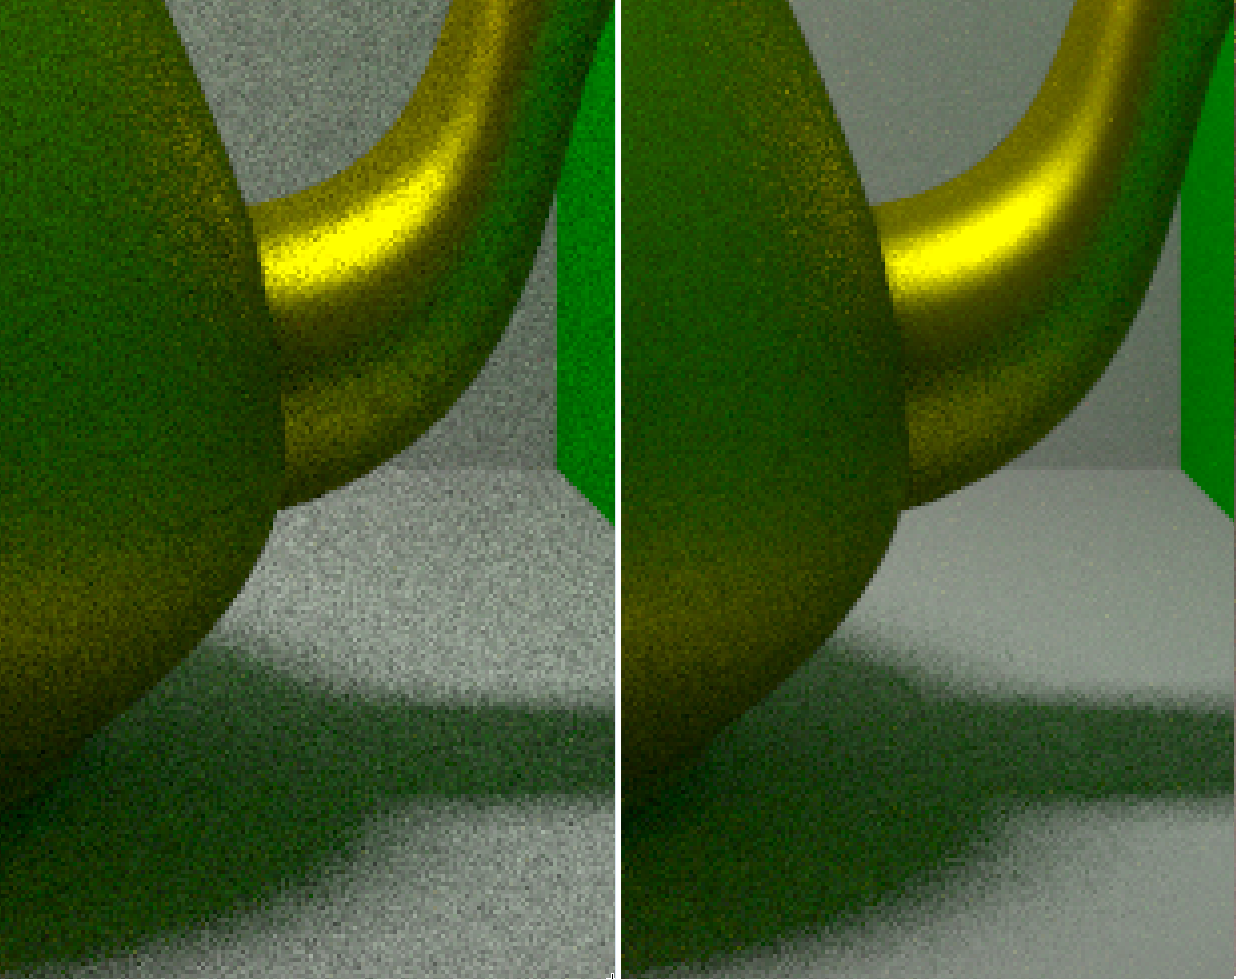
\includegraphics[width=1.0\linewidth]{images/qmc2.png}
	\caption{Pseudo random numbers (left) vs low discrepancy quasy random (right).}
	\label{fig:box2}
\end{figure}

\subsection{Pipelined execution}

The pipelined execution of our contribution scheme is drawn on figures \ref{fig:box3} and \ref{fig:box4}. For demonstration puprose we depicted PT and LT for only 2 ray bounce and simplified set of kernels (trace, shade, next\_bounce) is used per bounce. In fact our implementation run 7 different kernels per bounce, but this is not essential for the description of our idea. The difference between Path Tracing (fig. \ref{fig:box3}) and Light Tracing (fig. \ref{fig:box4}). The Copy and Contribute (paragraph 6 and 7) are represented by a green rectangle.


\begin{figure}[htb]
	\centering
	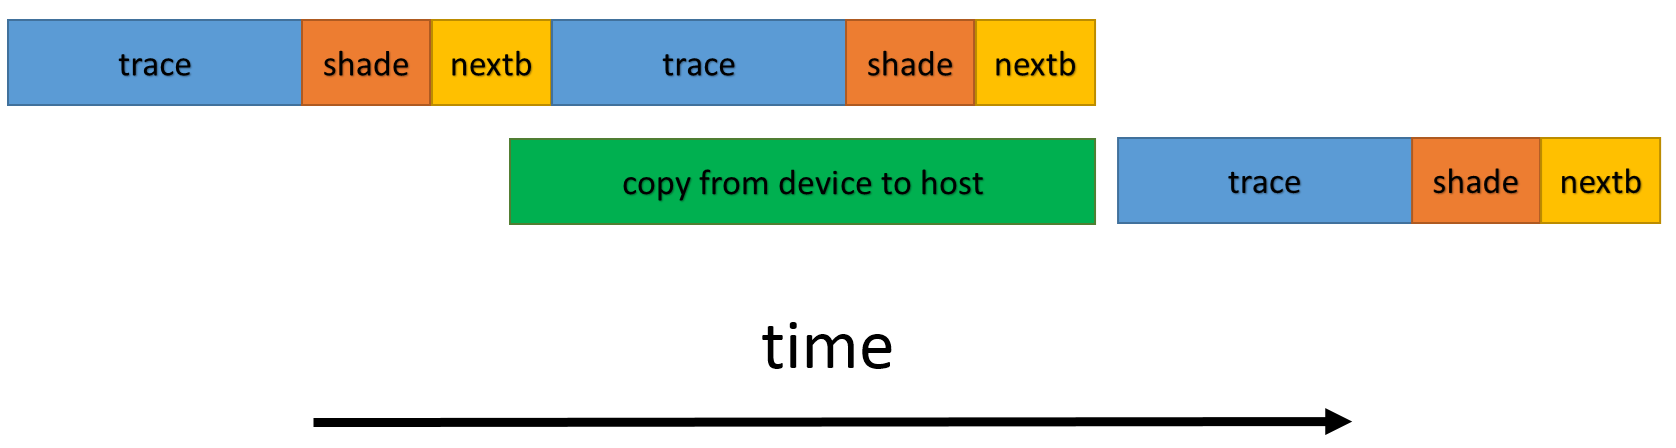
\includegraphics[width=1.0\linewidth]{images/pipeline1.png}
	\caption{Path Tracing pipeline.}
	\label{fig:box3}
\end{figure}

\begin{figure}[htb]
	\centering
	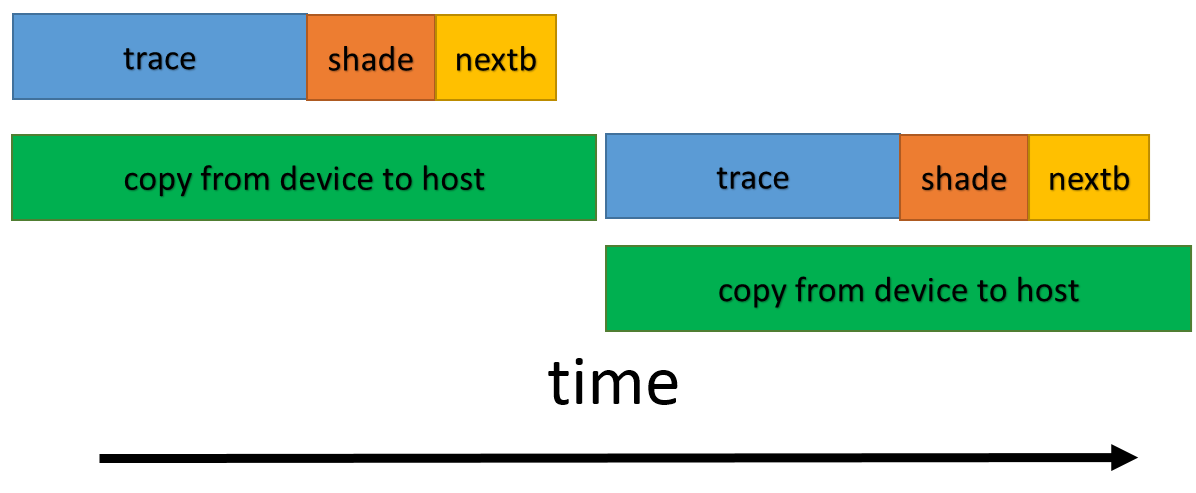
\includegraphics[width=1.0\linewidth]{images/pipeline2.png}
	\caption{Light Tracing pipeline.}
	\label{fig:box4}
\end{figure}


\subsection{Multiple GPUs}

\subsection{Multiple workstations}

\subsection*{Page Numbering, Headers and Footers}
Do not include headers, footers or page numbers in your submission. These will be added when the publications are assembled.

\begin{figure}[htb]
    \centering
    \rule{6cm}{3cm}
    \caption{Insert caption to place caption below figure.}
    \label{fig:box}
\end{figure}

\begin{table}[htb]
	\centering
	\begin{tabular}{|l|l|l|l|}
	\hline
	Graphics & Top & In-between & Bottom \\
	\hline
	Tables & End & Last & First \\
	\hline
	Figures & Good & Similar & Very well \\
	\hline
	\end{tabular}
	\caption{Table captions should be placed below the table}
\end{table}

\section{Figures/Captions}
Place Tables/Figures/Images in text as close to the reference as possible (see Fig.\ref{fig:box}). It may extend across both columns to a maximum width of 16 cm (6.3"). Captions should be Times New Roman 10-points.  They should be numbered (e.g., "Table 1" or "Figure 2"), please note that the word for Table and Figure are spelled out. Figure's and Table's captions should be centered beneath the image, picture or a table.

\section{Sections}
The heading of a section should be in Times New Roman 12-point bold in all-capitals flush left with an additional 6-points of white space above the section head.  Sections and subsequent sub- sections should be numbered and flush left. For a section head and a subsection head together (such as Section 3 and Subsection 3.1), use no additional space above the subsection head.

\subsection{Subsections}
The heading of subsections should be in Times New Roman 12-point bold with only the initial letters capitalized. (Note: For subsections and subsubsections, a word like the or a is not capitalized unless it is the first word of the header.)

\subsubsection{Subsubsections}
The heading for subsubsections should be in Times New Roman 11-point italic with initial letters capitalized and 6-points of white space above the subsubsection head.

\section{Acknowledgments}
Our thanks to ACM SIGCHI and SIGGRAPH for allowing us to modify templates they had developed.

%-------------------------------------------------------------------------
% example of algorithm typesetting
% to allow this, uncomment line 
% \RequirePackage[noend]{myalgorithm}
% in the wscg.sty file
% and download that package from Gabriel Zachmann's page http://zach.in.tu-clausthal.de/latex/
%
%
%\begin{algorithm}
%\hrule
%  \centering
%\begin{algorithmic}
%    \STMT $d_{l,r} = f_B(P_1), f_B(P_n)$
%    \WHILE{ $|d_l| > \epsilon $ and $|d_r| > \epsilon $ and $l<r$}
%        \STMT $d_x = f_B(P_x)$
%        \IF{ $d_x < 0$ }
%            \STMT $l, r = x, r$
%        \ELSE
%            \STMT $l, r = l, x$
%        \ENDIF
%    \ENDWHILE
%\end{algorithmic}
%\hrule
%\caption{Example of some pseudo-code}
%\label{fg:code}
%\end{algorithm}


%-------------------------------------------------------------------------

\begin{thebibliography}{99}
\label{references}
\bibitem[Kajiya86]{Kajiya86} James T. Kajiya. 1986. \textit{The rendering equation.} // In Proceedings of the 13th annual conference on Computer graphics and interactive techniques (SIGGRAPH '86), David C. Evans and Russell J. Athay (Eds.). ACM, New York, NY, USA, 143-150. DOI=http://dx.doi.org/10.1145/15922.15902

\bibitem[Antwerpen11]{Antwerpen11} Dietger van Antwerpen. 2011. \textit{Improving SIMD efficiency for parallel Monte Carlo light transport on the GPU.} In Proceedings of the ACM SIGGRAPH Symposium on High Performance Graphics (HPG '11), Stephen N. Spencer (Ed.). ACM, New York, NY, USA, 41-50. DOI: https://doi.org/10.1145/2018323.2018330 

\bibitem[Frolov et. all 2011]{frolov11} Frolov V., Kharlamov A., Ignatenko A. 2010. \textit{Biased Global Illumination via Irradiance Caching and Adaptive Path Tracing on GPUs.} Proceedings of GraphiCon'2010 conference. Moscow, Russia. pp 49-56.

\bibitem[Harris07]{Harris07} Mark Harris. 2007. Optimizing Parallel Reductiion in CUDA. // NVIDIA technical presentation.

\bibitem[Veach98]{Veach98} Eric Veach. 1998. \textit{Robust Monte Carlo Methods for Light Transport Simulation.} Ph.D. Dissertation. Stanford University, Stanford, CA, USA. Advisor(s) Leonidas J. Guibas. AAI9837162. 

\bibitem[Georgiev et. all 2012]{Georgiev12} Iliyan Georgiev, Jaroslav Krivanek, Tomas Davidovic, and Philipp Slusallek. 2012. \textit{Light transport simulation with vertex connection and merging.} ACM Trans. Graph. 31, 6, Article 192 (November 2012), 10 pages. DOI=http://dx.doi.org/10.1145/2366145.2366211 

\bibitem[Veach and Guibas 1997]{Veach97} Eric Veach and Leonidas J. Guibas. 1997. \textit{Metropolis light transport.} In Proceedings of the 24th annual conference on Computer graphics and interactive techniques (SIGGRAPH '97). ACM Press/Addison-Wesley Publishing Co., New York, NY, USA, 65-76. DOI=http://dx.doi.org/10.1145/258734.258775 

\bibitem[Kelemen et. all 2002]{Kelemen02} Csaba Kelemen, Laszlo Szirmay-Kalos, Gyorgy Antal and Ferenc Csonka. \textit{Simple and Robust Mutation Strategy for Metropolis Light Transport Algorithm.} EUROGRAPHICS 2002. Volume 21 (2002), Number 3.

\bibitem[Hachisuka et. all 2014]{Hachisuka14} Toshiya Hachisuka, Anton S. Kaplanyan, and Carsten Dachsbacher. 2014. Multiplexed metropolis light transport. ACM Trans. Graph. 33, 4, Article 100 (July 2014), 10 pages. DOI: https://doi.org/10.1145/2601097.2601138 

\bibitem[Bratincevic10]{VRayDMC} Toni Bratincevic. 2010. \textit{Demystifying V-Ray DMC Sampler} WEB publication. https://www.interstation3d.com/tutorials/ \newline vray\_dmc\_sampler/demistyfing\_dmc.html


\bibitem[Bogolepov et. all 2013]{Bogolepov13} Bogolepov D.K., Sopin D., Uljanov D. 2013. Turlapov V.E. \textit{GPU-Optimized Bi-Directional Path Tracing.} WSCG 2013 proceedings. Plzen. Czech Republic.

\bibitem[Popov et. all 2013]{PCBPT} Stefan Popov, Ravi Ramamoorthi, Fredo Durand, and George Drettakis. 2015. \textit{Probabilistic connections for bidirectional path tracing.} In Proceedings of the 26th Eurographics Symposium on Rendering (EGSR '15). Eurographics Association, Aire-la-Ville, Switzerland, Switzerland, 75-86. DOI=http://dx.doi.org/10.1111/cgf.12680 

\bibitem[Pharr2010]{PBRT} Matt Pharr and Greg Humphreys. 2010. \textit{Physically Based Rendering, Second Edition: From Theory to Implementation (2nd ed.).} Morgan Kaufmann Publishers Inc., San Francisco, CA, USA.

\bibitem[Frolov and Galaktionov 2017]{MemCompactMLT} Frolov, V.A. and Galaktionov, V.A. 2017. \textit{Memory compact Metropolis Light Transport.} Programing Computer Software (2017) 43: 196. https://doi.org/10.1134/S0361768817030057

\bibitem[Suhorukov11]{atomicsCL} Igor Suhorukov. 2011. OpenCL 1.1: Atomic opera-tions on floating point values. WEB publication. http://suhorukov.blogspot.ru/2011/12/opencl-11-atomic-operations-on-floating.html


\bibitem[Novak et. all 2010]{BPTGPU} Jan Nov\'{a}k and Vlastimil Havran and Carsten Daschbacher. 2010. \textit{Path Regeneration for Interactive Path Tracing.} Eurographics 2010 - Short papers. Eurographics Association. pp 61--64.

\bibitem[Davidovic et. all 2014]{VCMGPU} Tomas Davidovic, Jaroslav Krivanek, Milos Hasan, and Philipp Slusallek. 2014. Progressive Light Transport Simulation on the GPU: Survey and Im-provements. ACM Trans. Graph. 33, 3, Article 29 (June 2014), 19 pages. DOI: https://doi.org/10.1145/2602144

\bibitem[Schmidt et. all 2016]{MMLTGPU} M. Schmidt., Oleg Lobachev., Michael Guthe. 2016. \textit{Coherent metropolis light transport on the GPU using speculative mutations.} Journal of WSCG, 2016, vol. 24. no. 1 pp. 1--8.

\bibitem[Laine and Karras 2011]{Laine11} Samuli Laine, Tero Karras. 2011. High-performance software rasterization on GPUs. High-Performance Graphics 2011, August 2011. 

\bibitem[Sobol67]{Sobol67} Sobol I. M. 1967. Distribution of points in a cube and approximate evaluation of integrals. U.S.S.R. Comput. Maths. Math. Phys. 7: 86-112. 

\bibitem[Morton66]{Morton66} G. M. Morton. 1966. A Computer Oriented Geodetic Data Base; and a New Technique in File Sequenc-ing. In Research Report, IBM Ltd, ON, Canada

\end{thebibliography}

{\bfseries
Last page should be fully used by text, figures etc. Do not leave empty space, please. 

Do not lock the PDF -- additional text and info will be inserted, i.e. ISSN/ISBN etc. 
}


\end{document}

